
\documentclass[11pt, a4paper]{article}
\usepackage{fullpage}
\usepackage{graphicx}
\begin{document}

\title{Dynamische und statische Messung des Elastizitätsmoduls\\M15\\29.11.18}
\author{Janosch Ehlers, Piet Braasch}
\maketitle

\begin{center}
\textsc{Inhalt}
\end{center}

\begin{enumerate}
\item Ziel des Versuches
\item Theoretischer Hintergrund
\item Versuchsaufbau und -Durchführung
\item Statische Messung
\item Dynamische Messung
\item Messprotokoll
\item Anhang
\end{enumerate}

\newpage
\section{Ziel des Versuches}
Bestimmung des Elastizitätsmoduls, verschiedener Materialien, über die Ausbreitungsgeschwindigkeit von Schallimpulsen in Stäben mithilfe eines Piezoelements. Und der statischen Bestimmung des Elastizitätsmoduls durch Deformation einseitig eingespannter Stäbe mit diskreten Belastungen. 

\section{Theoretischer Hintergrund}
,,Mechanik der deformierbaren Medien'' ist ein Teilgebiet der Physik, welche sich mit den elastischen Eigenschaften von körpern beschäftigt. Durch elastische Verformung ist es nicht möglich einen Feststoff nachhaltig in seiner Struktur zu verändern. Bei einer plastischen Verformung ist dies der Regelfall. Diziplin dieses Teilgebietes ist die Errechnung von Elastizitätsmodul (E), Torsionsmodul (G) und Kompresionsmodul (K). Zu untersuchen ist das Elastizitätsmodul verschiedener Materialien (Aluminium, Eisen, Messing, Polycarbonat), dynamisch über Messung der Schallgeschwindigkeit in den Materialien und statisch über Biegung der Materialien. Schallwellen breiten sich in Festkörpern sowohl in Longitudinalwellen als auch in Transversalwellen aus. Außerdem ist die Schallausbreitung in Festkörpern schneller, da eine größere Bindung zwischen den Atomen besteht, als im Vergleich zu Gasphasen. Die Schallausbreitung ist abhängig von den elastischen Eigenschaften und der Dichte eines Materials. Wenn Dichte = $\rho$ dann gilt: $$v=\displaystyle{\sqrt{\frac{E}{\rho}}}$$ Für die dynamische Bestimmung des Elastizitätsmoduls wird der Stab mit Schallimpulsen versetzt, diese können durch ein Piezoelement gemessen werden. Der Abstand der Gemessenen Schwingungen kann in die Ausbreitungsgeschwindigkeit umgerechnet werden. Für die Statische bestimmung des Elastizitätsmoduls werden die Stäbe einseitig horizontal eingespannt. Das freie Ende wird hierbei durch eine Kraft $F$ belastet. Und der Stab um den Biegepfeil abgesenkt. Bei kleinem Biegepfeil bleiben die Querschnitte eben, sodass das Hook'sche Gesetzt gilt. Die durchbiegung eines Trägers nimmt mit der dritten Potenz seiner Länge $L^3$ zu. Und der Biegepfeil hängt vom Profil des Träger ab, welches in diesem Fall durch das sogenannte Flächen Trägheitsmoment $I=\frac{\pi}{4}\cdot R^4$ beschrieben wird. Es gilt: $$s=\frac{F}{3EI}\cdot L^3$$

\section{Versuchsaufbau und -Durchführung}
Zur Dynamischen bestimmung des Elatizitätsmoduls wurde das zu untersuchende Objekt mit einem Holzstab in schwingung versetzt. Mittels eines Piezoelements wurden dann die Schwingungen gemessen und mit ser Computer Software CASSY ausgewertet. Der Stab wurde dabei auf das Piezoelement gestellt und angeschlagen. Der Versuchsaubau der Statistische Messung des Elastizitätsmoduls bestand aus einem an der Wand eingespanntem Stabes und der behängung des freiliegenden Endes durch Gewichte. Mithilfe eines Lasers wurde auf einem enferntem Schirm die Auslenkung des Stabes aus der Ruhelage abgebildet. Durch Variation der Gewichte von 50g bis 1050g kann die Kraft Diskret bestimmt werden. Wie in den Skizzen Fig. 4, Fig. 5 zusehen. \newpage


\section{Statische Messung}

In Tab. 1 können die gemessenen Werte von des Statischen Verfahrens eingesehen werden. Da gilt: $$s=\frac{FL^3}{3EI}$$ mit $I=\frac{\pi}{4}\cdot R^4$. Da $s$ dem Biegepfeil entspricht und nicht dem gemessenen Wert nach dem Versuchsaufbau, muss $s$ mithilfe des Strahlensatzes $\frac{a}{b}=\frac{c}{d}$ (siehe Fig.5) umgerechnet werden. Wenn gilt: $Laenge_{Fixpunkt,Schirm} := l_{ges}$, $Laenge_{Stange} := b$ und $Abstand_{Nullmessung, Messung n} := y$ dann kann folgende Gleichung aufgestellt werden: $$s=\frac{yb}{l_{ges}}$$ $$\frac{yb}{l_{ges}}=\frac{FL^3}{3ER^4\frac{\pi}{4}}$$ oder $$\frac{yb}{l_{ges}}=\frac{4FL^3}{3ER^4\pi}$$ Da wir E suchen wird nach E umgestellt: $$\left.\frac{yb}{l_{ges}}=\frac{4FL^3}{3ER^4\pi}\ \right|\cdot E$$ $$\left.\frac{Eyb}{l_{ges}}=\frac{4FL^3}{3R^4\pi}\ \right| \cdot l_{ges}$$ $$\left. ybE=\frac{4FL^3l_{ges}}{3R^4\pi}\ \right| \cdot \frac{1}{yb}$$ $$E=\frac{4FL^3l_{ges}}{3ybR^4\pi}$$ Nach einsetzen der Werte in die Formel kommen wir auf die Werte, wie in Tab. 2 zusehen.\\
Daraus können wir nun Mittelwert und Fehler berechnen:\\

\begin{tabular}{r|ccc}
 & $Aluminium_{(pa)}$ & $Messing_{(pa)}$ & $Eisen_{(pa)}$\\
Mittelwert & 224800185497,967	& 495174523324,915	& 819882877639,469\\
Varianz & $\pm 10704770737,9984$	 & $\pm 23579739205,9482$	& $\pm 39042041792,3555$\\
\end{tabular}\\
\begin{flushleft}
Aluminium: $(224800185497,967Pa \pm 10704770737,9984Pa)$\\
Messing: $(495174523324,915Pa \pm 23579739205,9482Pa)$\\
Eisen: $( 819882877639,469Pa \pm 39042041792,3555Pa)$\\
\end{flushleft}
Ein Diagramm indem s über F für jedes Material abgebildet wurde ist bei 6.0 Messprotokoll unter Fig. 1, Fig. 2, Fig. 3 zu finden. 

\newpage
\section{Dynamische Messung}

\begin{center}
\textsc{Eisen}
\end{center}

Im Anhang 1 (A1) sieht man die Messkurve von Schallimpulsen in einer Eisenstange, hierbei ist die Zeit $t_{(ms)}$ in Abhängigkeit von der Spannung $UA1_{(V)}$ dargestellt. Zunächst lässt sich beobachten, dass der Graph zu beginn der Aufzeichnung eine starke Intensität hat, welche bereits nach kurzer zeit, ca. 40ms nachlässt. Beim heranzoomen an den Graphen lässt sich starkes Übersteuern erkennen. Die Wellenkämme flachen immer weiter ab und das Übersteuern nimmt auch ab. Unsere Messwerte sind aus dem Bereich zwischen 63-69ms, da hier beinahe keine Übersteuerung mehr zu erkennen ist und Schwingung beinahe harmonisch ablaufen. Bei Messwerten aus anderen Bereichen mit mehr übersteuerung oder großen unterschieden zwischen den einzelnen Amplituden würden wesentlich ungenauere Werte ergeben.   

\begin{center}
\textsc{Polycarbonat}
\end{center}

In Anhang 2 (A2) sieht man die Messkurve von Schallimpulsen in einer Stange aus Polycarbonat, hierbei ist die Zeit $t_{(ms)}$ in Abhängigkeit von der Spannung $UA1_{(V)}$ dargestellt. Genau wie bei der Eisenstange lässt sich zu beginn eine starke Intensität der Welle beobachten, im Gegensatz zur Eisenstange hat die Welle von Polycarbonat eine Größere Wellenlänge, also weniger Perioden im gleichen Zeitraum. Auch hier lässt sich beim heranzoomen an der Graphen starkes Übersteuern feststellen. Der von und gewählte Zeitraum liegt zwischen 130-140ms, da hier eine beinahe Harmonische Schwingung zu erkennen ist und kein Übersteuern vorhanden ist.

\begin{center}
\textsc{Messing}
\end{center}

In Anhang 3 (A3) sieht man die Messkurve von Schallimpulsen in einer Messingstange, hierbei ist die Zeit $t_{(ms)}$ in Abhängigkeit von der Spannung $UA1_{(V)}$ dargestellt.  Auch bei der Messingstange lässt sich zu Beginn eine stärkere Intensität beobachten, welche im verlauf der Messung immer weiter abnimmt. Im Vergleich zu den Maximalen Auslenkungen der Graphen von Eisen und Polycarbonat, beide weit über $\pm 10V$ ist bei Messing die maximale Auslenkung nur bei ca. 8V. Auch hier lässt sich starkes Übersteuern beim heranzoomen erkennen. Der von uns gewählte Bereich liegt zwischen 30-50ms da hier wieder kaum übersteuern zu erkennen war und die Welle einer Harmonischen Schwingung ähnelt.

\begin{center}
\textsc{Aluminium}
\end{center}

In Anhang 4 (A4) sieht man die Messkurve von Schallimpulsen in einer Aluminiumstange, hierbei ist die Zeit $t_{(ms)}$ in Abhängigkeit von der Spannung $UA1_{(V)}$ dargestellt. Zu beginn der Messung weist auch die Welle der Aluminiumstange eine starke Intensität auf, welche aber nach kurzer Zeit nachlässt. Die maximale Auslenkung (<10V) ist zwar größer als bei der Messingstange, aber auch kleiner als bei der Polycarbonat oder der Eisenstange. Näher betrachtet erkennt man auch hier starkes Übersteuern. Der von uns gewählte Bereich liegt zwischen 65-75ms, da hier wieder kaum Übersteuern vorhanden war und die Schwingung sich beinahe Harmonisch verhält.

$$\left. \frac{\Delta V_L}{V_L}=\pm \left\{ \frac{\Delta L}{L} + \frac{\Delta t}{t} \right\}\ \right|  \cdot V_L$$
$$\Delta V_L=\pm \left( \frac{\Delta L}{L} + \frac{\Delta t}{t} \right)\cdot V_L$$
$$\Delta V_L=775,81 \frac{m}{s}$$
$$\left. \frac{\Delta \rho}{\rho}=\pm \left\{ \frac{\Delta m}{m} + \frac{\Delta L}{L} + \frac{2\Delta d}{d} \right\}\ \right|  \cdot \rho$$
$$\Delta \rho=\pm \left\{ \frac{\Delta m}{m} + \frac{\Delta L}{L} + \frac{2\Delta d}{d} \right\}\cdot \rho$$
$$\Delta \rho = 1090,43$$
$$\left. \frac{\Delta E}{E}=\pm \left\{ \frac{2\Delta V_L}{V_L} + \frac{\Delta \rho}{\rho	}\right\}\ \right| \cdot E$$
$$\Delta E=\pm \left\{ \frac{2\Delta V_L}{V_L} + \frac{\Delta \rho}{\rho	}\right\}\cdot E$$
$$\Delta E = 102,03 GPa$$

\textbf{Messing}

$$\Delta V_L = 462,67 \frac{m}{s}$$
$$\Delta \rho = 1186,04$$
$$\Delta E  = 45,95 GPa$$

\textbf{Polycarbonat}

$$\Delta V_L = 147,35 \frac{m}{s}$$
$$\Delta \rho = 112,52$$
$$\Delta E  = 69,29 MPa$$

\textbf{Aluminium}

$$\Delta V_L = 772,15 \frac{m}{s}$$
$$\Delta \rho = 328,17 $$
$$\Delta E  = 30,56 GPa$$

\textbf{Eisen}

$$\left. \frac{\Delta E}{E}=\pm \left\{ \frac{2\Delta V_L}{V_L}+\frac{\Delta\rho}{\rho}\right\}\ \right|\cdot E$$
$$\Delta E = \pm \left\{ \frac{2\Delta V_L}{V_L}+\frac{\Delta\rho}{\rho}\right\}\cdot E$$
$$\Delta E = 102,03 GPa$$

\newpage
\section{Messprotokoll}

\begin{center}
\textbf{Tab. 1}
\textsc{y über m}\\

\begin{tabular}{c|ccc}
$Gewicht_{(g)}$ & $Aluminium_{(mm)}$ & $Messing_{(mm)}$ & $Eisen_{(mm)}$ \\
\hline
50		&	7,5		&	7		&	3,5\\
100		&	15		&	12,5	&	6\\
150		&	22,5	&	18		&	9\\
200		&	30		&	24		&	11,25\\
250		&	37,25	&	30		&	14,25\\
300		&	44,75	&	35,5	&	16,75\\
350		&	51,25	&	41,25	&	19,25\\
400		&	59,25	&	46,25	&	21,75\\
450		&	66,25	&	51,5	&	24,25\\
500		&	74,25	&	58,5	&	27,25\\
550		&	81,75	&	64,25	&	29,75\\
600		&	88,75	&	69,25	&	32,75\\
650		&	96,5	&	74,25	&	35,75\\
700		&	104		&	80,5	&	38,25\\
750		&	111,5	&	85,5	&	40,75\\
800		&	119 	&	91		&	43,25\\
850		&	126,5	&	96,25	&	45,75\\
900		&	133,5	&	102,25	&	48,75\\
950		&	141,5	&	107,75	&	51,75\\
1000	&	149		&	113,25	&	54,25\\
1050	&	156,5	&	119,75	&	56,75\\

\end{tabular}\newpage

\textbf{Tab. 2}
\textsc{Wertetafel E über m}\\
\vspace{5mm}
\begin{tabular}{cccc}
$Gewicht_{(g)}$ & $Aluminium_{(pa)}$ & $Messing_{(pa)}$ & $Eisen_{(pa)}$\\
50 & 212293611210,424	& 2416104170439,55	& 4510061118153,83\\
100 & 212293611210,424	& 1353018335446,15	& 2067111345820,51\\
150 & 212293611210,424	& 939596066282,049	& 1378074230547,01\\
200 & 212293611210,424	& 704697049711,537	& 1202682964841,02\\
250 & 213718400547,407	& 544965718443,589	& 949486551190,281\\
300 & 213479609038,415	& 476414906847,236	& 740457795517,794\\
350 & 217471504166,776	& 355338148703,029	& 673580556607,391\\
400 & 214980872111,822	& 390059339948,44	& 518397829672,854\\
450 & 216299151044,583	& 306509008029,872	& 488202492171,291\\
500 & 214437991121,64	& 308380247395,134	& 579273905083,979\\
550 & 214241259019,694	& 263233139191,858	& 435846242510,665\\
600 & 215283662072,543	& 227945327271,313	& 344279474668,232\\
650 & 214493545005,351	& 235373560038,331	& 315388889381,387\\
700 & 214334895933,601	& 210096014820,831	& 368469045600,804\\
750 & 214197589786,302	& 197809698164,642	& 276690866144,407\\
800 & 214077591136,562	& 185854166956,889	& 286766891905,735\\
850 & 213971821575,724	& 175716666941,059	& 258773998582,597\\
900 & 214678932684,699	& 154378620181,305	& 277542222655,621\\
950 & 213793919416,858	& 167426862854,899	& 239665083573,392\\
1000 & 213718400547,407	& 149339772124,299	& 228620609676,001\\
1050 & 213650119908,254	& 141233646706,279	& 258285438484,581\\
\end{tabular}\newpage
\end{center}

\section{Anhang}

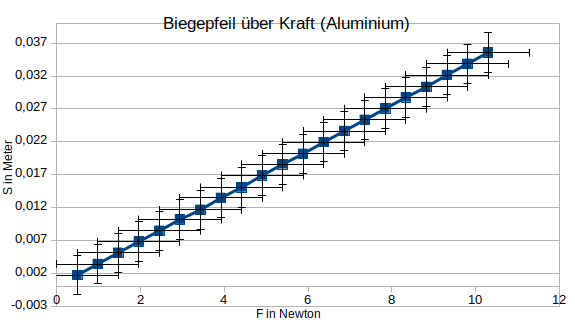
\includegraphics[scale=1]{bukA.png}\\
Fig. 1\\
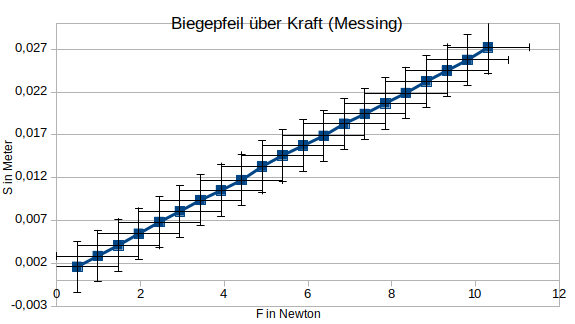
\includegraphics[scale=1]{bukM.png}\\
Fig. 2\\
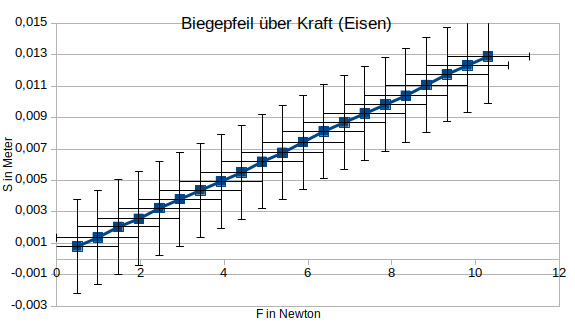
\includegraphics[scale=1]{bukE.png}\\
Fig. 3\\
\includegraphics[scale=0.7]{fig45.pdf}\\
Fig. 4 / 5\\
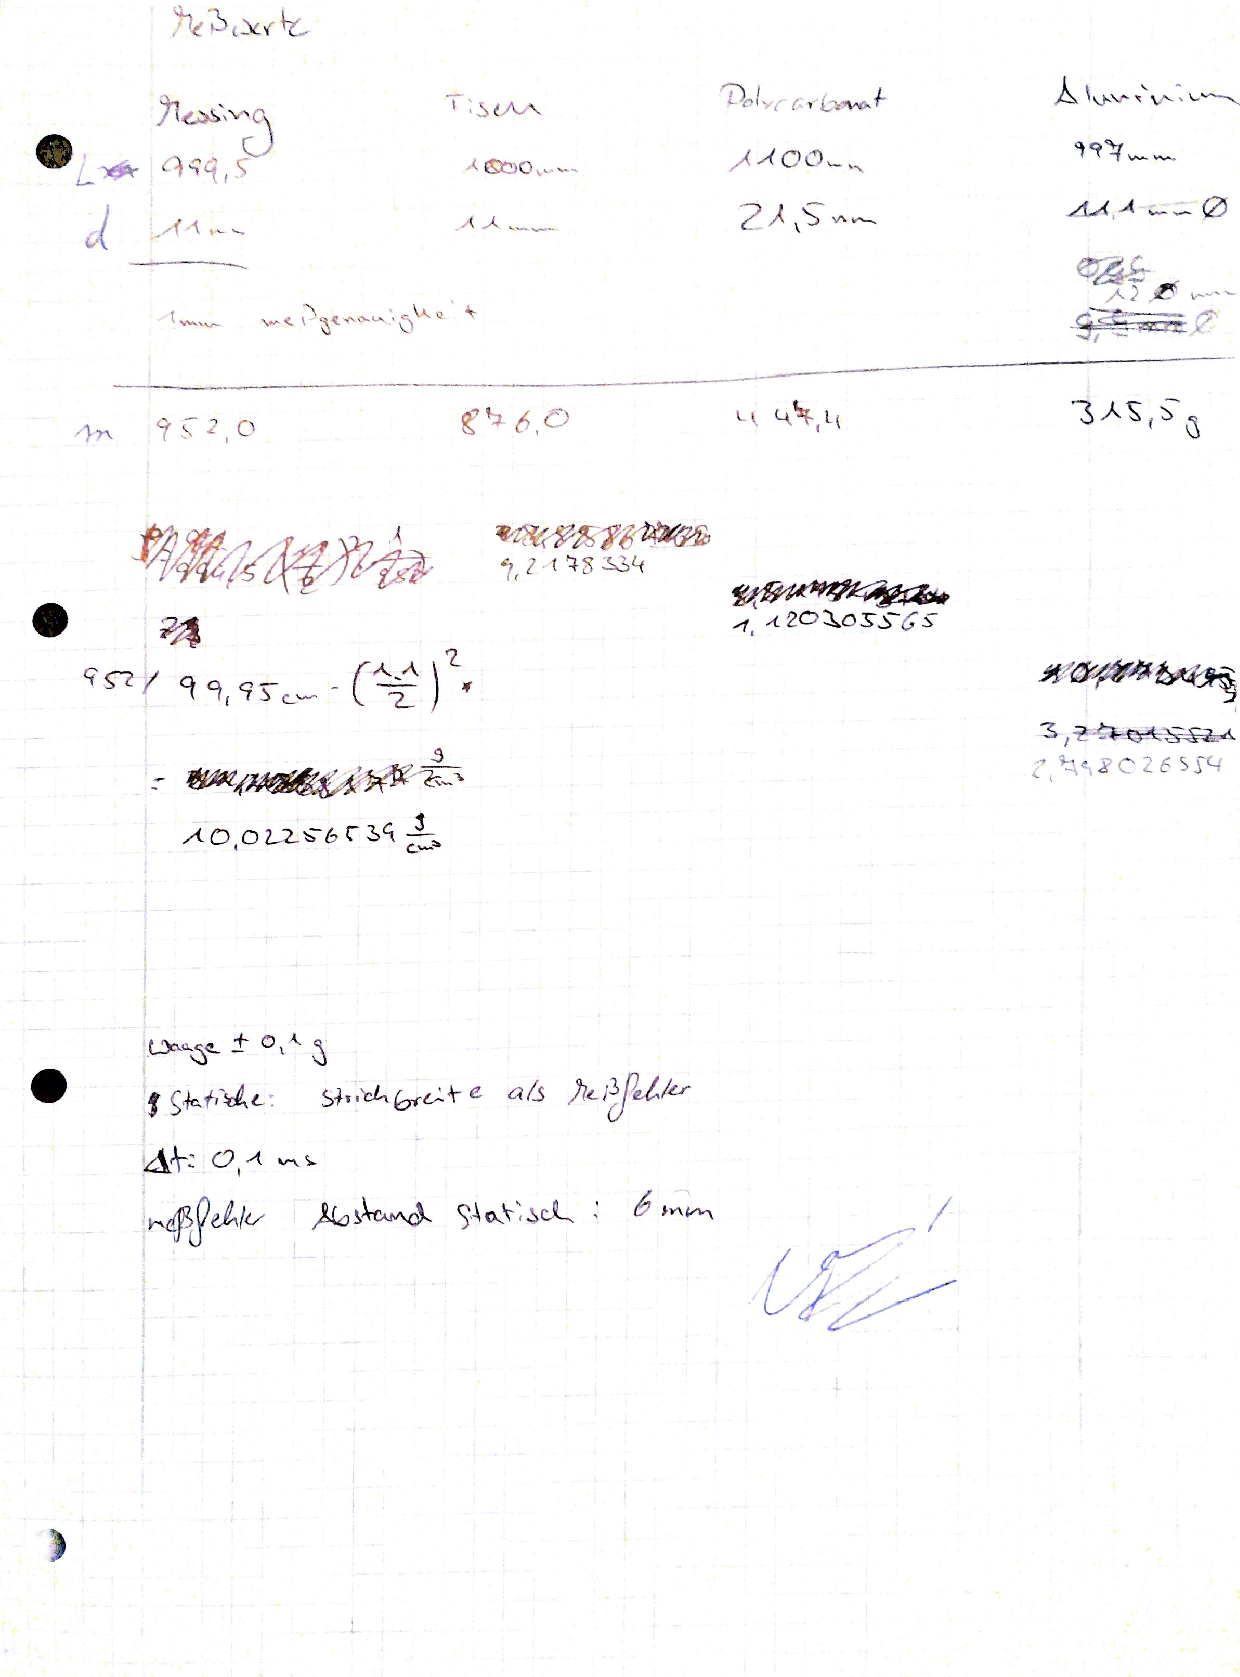
\includegraphics[scale=0.7]{Messdaten.pdf}\\


\end{document}
